\chapter{Simulations}
In this chapter, we detail simulations that we developed to test our hypothesis with a complete implementation of K-HAS. LORIS was implemented because current technology does not fully support the requirements of the K-HAS architecture, because of this we implemented a simulation of K-HAS that satisfies all of its requirements.

Using RePast, a java-based network simulation tool, we created a network to emulate K-HAS. Repast is an agent-based modelling system that allows for agents to be created and placed on a grid. Ticks denote a period of time and simulations can run for a fixed number of ticks, or until stopped. Ticks can also be used to schedule events, such as searching for neighbours, by calling methods that last for a set number of ticks, or begin at a particular tick. Similar to the chaining of rules we described with Drools, ticks are the core of Repast's scheduling mechanism which can be used to schedule single events, as well as chaining events. Consider a train simulation. A train may take three hundred ticks to arrive at its destination, from the train arrival a scheduled event to open doors and make announcements which could schedule other events and so on.

Agents are created, using the RePast SDK and Java classes are used to manipulate their behaviour. Simple networks may only contain basic agents with only a few variations from those provided by RePast. However, for more complex networks, a hierarchy of agents is required and Java's inheritance can then be used create subclasses of an agent.

A 2D (or 3D) space is used to display the grid and the simulation is run within Repast's own GUI, that provides functionality such as editing the properties of classes, integrating with Matlab, taking screenshots and saving different configurations of the same network.

The rest of this chapter is structured as follows. Section 2 describes the implementation of the network. Section 3 outlines the results and Section 4 compares these with LORIS and the current solution in our motivating scenario. Section 5 concludes our findings and highlights areas that require further experimentation.

\section{Implementation}\label{sim:imp}
	While the aim of these simulations were to show the effectiveness of K-HAS over the current solution, we also wanted to determine if it was the optimal solution, in terms of delivery of interesting data and in terms of network lifetime. The ideal solution would be to attach DP nodes to all cameras in the network, however the short battery life means that replacements would be made as often as the current manual solution. Because only one of these simulations matches K-HAS, the terminology used in this chapter is more generic and focussed on nodes that have knowledge but do not match our definitions of DP and DC nodes. Instead we use the term \textit{sensing node} to define a node that is capable of capturing an observation, \textit{routing node} to define a node that processes the data from sensing nodes and \textit{central node} to define the end point of the network, where data is made available to users. While these definitions are similar to DC, DP and DA nodes the key difference is that sensing and routing nodes possess have varying levels of knowledge processing capabilities, explained below:
	
	\begin{itemize}
		\item No Knowledge (NK): The node possesses no knowledge processing capabilities.
		\item Low Knowledge (LK): The node possesses basic knowledge processing capabilities and contains a static rule base.
		\item High Knowledge (HK): The node possesses high knowledge processing capabilities and is able to process data, metadata and use a dynamic rule base.
	\end{itemize}
	
	Using the results of the image processing application developed, explained in Section \ref{tech:sf:triton}, for the details of HK processing. Which means that it has 82\% accuracy at detecting TP images, with a 97\% accuracy for finding TN images. Nodes with LK do not have the ability to mark an image as empty, but they can mark an image as interesting. The results we have from out rule base are not as extensive as the results we have for Triton, so instead we use a predefined 10\% accuracy for detecting TPs. The scenarios we have implemented cover the possible combinations of HK, LK and NK, which we have outlined below:
	
	\begin{itemize}
		\item NK-ALL: Sensing and routing nodes possess no knowledge processing capabilities.
		\item LK- ALL: Sensing and routing nodes possess low knowledge processing capabilities.
		\item NK-LK: Sensing nodes possess no knowledge processing and routing nodes have low knowledge.
		\item LK-HK (K-HAS): Sensing nodes have low knowledge and routing nodes possess high knowledge.
		\item HK-ALL: Sensing and routing nodes have high processing capabilities.
	\end{itemize}

%\section{K-HAS Implementation}
%As described in Chapter \ref{chap:arch}, K-HAS consists of three tiers: Data Collection, Data Processing and Data Aggregation. The DC tier focusses on capturing sensed data, performing basic processing and routing sensed data to the DP tier. The DP tier has more knowledge-processing capabilities and nodes are responsible for processing sensed data. Using a rule engine and a dynamic knowledge base, DP nodes process more than just the metadata of sensed data in order to create a classification. DP nodes have a direct connection to the DA node, which is the the endpoint in the K-HAS network, an Internet connected node that stores all sensed data from the network and acts as the central knowledge base.

%K-HAS was originally intended to be deployed around Danau Girang and, over the course of three years, we have collected several thousand images and local knowledge interviews in order to configure K-HAS before deployment. Because of this, the data we have collected was used to create a deployment of K-HAS using scientific observations, in order to fit with our motivating scenario. LORIS had already been deployed to capture scientific observations, so this made a comparison of the three (current manual solution, LORIS and K-HAS simulation) possible and because we already had metrics on areas of the network such as battery life, transmission time of a Darwin Core archive and processing time.

Before implementing, we designed the agents required based largely on the existing ontology. Using that, we created a hierarchy of nodes inheriting common properties from a node object. As previously mentioned, we had metrics on range and transmission times from previous experiments and the deployment of LORIS, we used these to create properties for each transmission medium that could be used by each node object.

We also needed to create an object to represent the DwC archives, a Drools REST API had been implemented to work with the LORIS web interface, and much of the DwC archive code was reusable within RePast. 

The structure of the simulation is shown below. Network builder instantiates all the nodes, places them on randomly on the grid and schedules events once the simulation has started. The nodes then use the properties of their transmission medium to find nodes in range and create a connection, depicted by a line between the node. The simulation uses metrics extracted from the images taken at Danau Girang, but the chance of an image being captured at a camera is based on the average capture rate of a camera. The fire rate has been calculated by the average number of pictures captured in a day taken by each camera. Figure \ref{fig:sim} shows an example simulation of the LK-HK scenario.


	\begin{figure}[h]
	\centering
	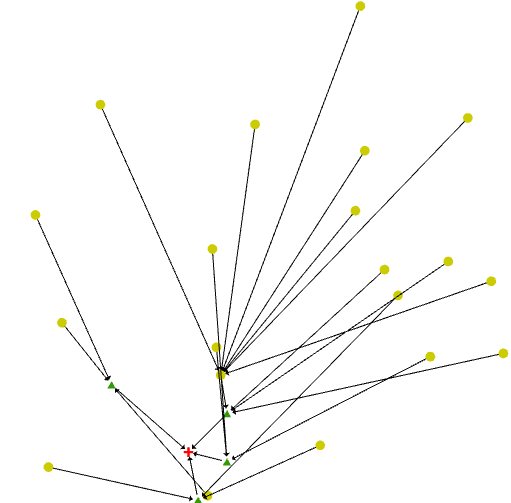
\includegraphics[width=0.70\textwidth]{Chap7/figures/khas_sim}
	\caption{K-HAS Simulation}
	\label{fig:sim}
	\end{figure}

%DG mode means that it models a 6 month deployment in Danau Girang from 2010. All images taken in that time had the time they were taken, the original camera ID and the size of each image recorded into a CSV file. This file is read by the Network Builder and the contents are provided to each node. The first tick starts at the same time as the first image is taken. The number of deployed nodes matches the number of deployed cameras and, upon each tick, they check whether an image was taken by them at that tick. If so, an image is captured, archived and forwarded to the nearest DP node. This process runs, using the scheduler in RePast, for the six month deployment and the details of each archive (time captured, size, route taken, time taken to reach DA node) is saved into a CSV file when it reaches the DA node. Once the six month deployment has run, the simulation can either stop or continue randomly.



\begin{itemize}
\item Network Builder
\item Node
	\begin{itemize}
	\item Sensing
	\item Routing
	\item Central
	\end{itemize}
\item Darwin Core
	\begin{itemize}
	\item Identification
	\item Location
	\item Occurrence
	\item Image
	\item Species
	\end{itemize}	 
\end{itemize}

\subsection{Darwin Core}
The Darwin Core class represents a DwC archive, encapsulation Identification, Location, Occurrence, Image and Species. The images we have collected from Danau Girang were processed to find details such as the average size when taking at night and day, how often an average camera triggers and the percentage of images with animal content. These data were then used to specify how often a randomly placed node should capture an observation per tick.

Upon each capture, and based on the `time' of day, images are created, given a random size based on the maximum and minimum size found in the 120,000 images collected from DG and the sum of the images is used to calculate the size of the archive. Using this size, a DC node calculates how long the archive takes to send based on the size and the transmission rate, we assume that the rate stays constant for the duration of transmission.
When an archive is sent to the DP node, we used the average time for our image processing tool and Drools engine to run and attempt a classification, which is 143 seconds (ticks). To keep the classifications as general as possible, so that the simulation applies to any WSN for scientific observations, archives are not classified down to the species level, they are marked as \textit{interesting} or \textit{empty} and then forwarded to the DA node.

\subsection{Routing}
The routing protocol used by K-HAS needs to be dynamic in order to adapt to nodes being added and removed during deployment, while minimising traffic in a resource constrained network. The approach we use a modification the Minimum Cost Forwarding Algorithm (MCFA), described in Section \ref{bg:rp}. A cost is assigned to each node, based on how far they are from the central node, with neighbouring nodes choosing to connect to the node with the lowest cost. However, in normal implementations of MCFA, all nodes are of the same type and simply need to connect to a base station. This protocol is used in all scenarios.

In K-HAS, DC nodes cannot connect directly to a DA node, because processing would not take place. K-HAS MCFA works with a discovery phase and a transmission phase. The discovery phase is a scheduled event, taking place at the start of deployment but it can be run throughout deployment to react to nodes being added or removed. 

\subsubsection{Discovery}
	Discovery begins at each central node, scanning nodes in range for routing nodes and sending a broadcast packet with a cost of 0 to inform them that they are within range of a central node which, in our implementation, uses Wi-Fi. Once received, routing nodes increment the count and forward the packet to any routing nodes within range of them, where we use the range of Digimesh. We found that this method overloaded the routing nodes and all sensing nodes within range would connect to the first routing node they receive the broadcast from. We then implemented a method, called \textit{load balancing}, which uses the sensing nodes connected to a routing node to calculate whether it should offload new nodes to a neighbouring routing node.
	
	The maximum connections a routing node can have is determined by the total number of sensing nodes in the network divided by the total number of routing nodes, which is held in the knowledge base of the central node. Once a routing node has the maximum number of connections allowed, it starts to offload to a neighbouring routing node that is also in range of the sensing node requesting a connection. If there are no neighbouring nodes then it simply goes over the maximum number of connections allowed, to save sensing nodes being left with nowhere to send their data.
	
	If the sensing node that receives the broadcast does not have an existing route to a central node, or the cost of the current route is higher than the received route, it adds an edge to the routing node, increments the count and forwards it to all nodes in range. This process continues until the broadcast reaches the edge of the network. Nodes do not have global knowledge of the route to the central node, only of their neighbour with the lowest cost.
	
	This phase can be repeated throughout the course of the deployment, simply by scheduling it as an event to occur every \textit{n} ticks. However, the simulation currently only uses the discovery phase at the beginning of the deployment.
	
\subsubsection{Transmission}
	Once the discovery phase has been completed, providing nodes are within range of the DA node, the transmission phase begins where only DwC archives are then sent across the network. Observations are captured based on the mode of the simulation and sent to the lowest cost neighbour.
	
	In order to manage transmissions, sensing nodes have a \textit{SendState} object that contains the next archive to send, the time to send it and whether it is currently sending. This is used to determine what operations to perform, once an archive has been sent, it is delete from the SendState and the sending flag is set to false. A new archive is then added and sent when the opportunity arises.
	
	When a routing node receives the archive, it begins processing and we have implemented both sending and processing as serial processes. Routing nodes use the SendState as well, but they do not add any archive, they add an archive once it has been processed and they then select the oldest archive that has been classified as interesting, providing that an archive is not already waiting to be sent. The archive stores information about the route it takes, recording every hop, as well as the time it took from capture to central node.
	
	Scheduled sending events run every thousand ticks, which is configurable, to check the sending state of the node and send any archives in the SendState. The node then waits for the number of ticks that it will take in order to transmit the archive.
	
	Once the simulation is completed, either manually or through a defined number of ticks, the archives in each central node are iterated over and written to a CSV file, with details like the path it took, total transmission time and time of capture.
	
\subsection{Capture}
	Using the existing data collected from Danau Girang, we calculated how often a camera triggers in a six month deployment, as well as how often the observation contained interesting content. 
	
	To calculate the count of interesting images, we processed every directory of images to extract the largest object in the foreground, using our Triton program. Once processed, we iterated through every directory, counted the total number of images and the total number of extracted images. We then calculated the average for each directory and then summed those averages divided by the total number of directories. This gave us a 20.7\% chance of an image being interesting.
	
	The chance of camera trigger was calculated by the total number of observations (13,399) divided by the number of seconds in six months (15,552,000). This gives a chance of 0.000861561. A random number is generated every and compared to this, if the value is fewer than or equal to the chance, then an observation is captured.

\section{Results}

	In this section, we explain the results for each scenario that we detailed in Section \ref{sim:imp}. Each scenario was run 100 times, with each run lasting a six month deployment, and the results of each run is written to a CSV file. We then process all of the CSV files for each scenario and extract the duration for all observations, as well as metrics for observations marked as interesting and empty. Table \ref{tab:observ_int} and \ref{tab:observ_empty} show the transmission data for each scenario, aside from NK-ALL, and it is clear that HK-ALL is the most effective implementation. With knowledge on every node, HK-ALL is able to detect interesting observations right at the edge of the network and prioritise them through every node, giving an average duration of 83 hours for interesting observations. Perhaps more important is that 90.92\% of all interesting observations were true positives.

	As knowledge is pushed out further to the edge of the network, the trend of reduced transmission time is clear and there is a significant drop in the duration of interesting observations. Another pattern to be observed here is that the percentage of empty images received by the central node decreased when there is more knowledge-processing capabilities, also meaning that the percentage of interesting observations increases.

	With the increase of interesting observations there is an increase in the ratio of TP to FP images. A network with solely HK nodes results in nearly 91\% of all interesting images as TP. Although our implementation of K-HAS is only short of this by 1.8\%. This difference is minimal when the number of long life LK nodes are taken into account. These simulations prove that K-HAS is the best solution when many of the sensing nodes are placed in locations that are not easily accessible, allowing for a lifetime of 4 months or more; using the more capable HK nodes would mean that batteries would need to be replaced every 3 weeks. Relating this to our motivating scenario, nodes deployed more than a kilometre into thick rainforest are not easily accessible.




	
	
\begin{table}[h]\footnotesize
\centering
\begin{tabular}{| c | c | c | }
\hline
Mode  & Avg. Duration \\
\hline
NKALL & 730 \\
NKLK  & 539 \\
LKALL & 649 \\
LKHK  & 454 \\
HKALL & 475 \\
\hline
\end{tabular}
\caption{Simulation Results}\label{tab:observ}
\end{table}

\begin{table}[h]\footnotesize
\begin{tabularx}{\textwidth}{ |X|X|X|X|X|X|X| }
\hline
Mode & Avg. Interesting Duration & \% Interesting & \% TP & \% FP \\
\hli
NKLK & 753 & 21.36 & 15.41 & \\
LKALL & 523 & 22.46 & & \\
LKHK & 257 & 27.36 & 89.1 & 10.9 \\
HKALL & 83 & 33.19 & 90.92 & 9.08 \\
\hline
\end{tabularx}
\caption{Simulation Results for Interesting Observations}\label{tab:observ_int}
\end{table}

\begin{table}[h]\footnotesize
\begin{tabularx}{\textwidth}{ |X|X|X|X|X|X|X| }
\hline
Mode & Avg. Empty Duration & \% Empty & \% TN & \% FN \\
\hline
NKLK & 834 & 78.64 & &  \\
LKALL & 686 & 77.54 & & \\
LKHK & 646 & 72.64 & 95.51 & 4.49 \\
HKALL & 670 & 66.81 & 93.69 & 6.31 \\
\hline
\end{tabularx}
\caption{Simulation Results for Empty Observations}\label{tab:observ_empty}
\end{table}
	
\section{Improvements}
Although the simulations do show an improvement over the current implementation, there are features that could be added to ensure that the simulation models a real-world implementation as closely as possible. Currently, the processing time of DP nodes is based on the average time to process an archive, using a random time within a range would make this less static. 

All nodes within the network do not use a battery life and, due to the short deployment time of LORIS, we do not have accurate information on how long batteries last on each node. This is most important on DC nodes as there may be hundreds deployed at any one time and the DA node must report when a DC node does not report for a while. This also goes for transmission, using a fixed range and transfer rate suits a dynamic network in an open environment but obstacles and weather affect the rate and this could be taken into account in a future implementation.

In our implementation of K-HAS, we are using image-based scientific observations but the chance of a camera being triggered is the same for every DC node. In a future version, it would be more realistic to use different chances of triggering based on the cameras location, or based on random assignments. However, we believe that a more general, extensible simulation that was able to handle many different types of sensed data would be the truest model of K-HAS; using property files, as we currently do, to provide details on the sensed data, processing times and a knowledge base.

\section{Conclusion}
In this chapter we have detailed the development and results of our simulation of the K-HAS architecture. Current technology limits the implementation of the original architecture we developed, so using a simulation framework is the best alternative. We have modelled all variables based on existing data from our motivating scenario and results have shown that using knowledge bases on deployed nodes for the processing of observations within the network allows `interesting' sensed data to be prioritised and delivered to a DA node more than four hundred hours earlier than a manual solution; which does not include human processing time.

While the simulation is not feature complete, we believe it is accurate enough to show how K-HAS utilises the knowledge-processing capabilities at each tier to process, and prioritise, sensed data based on knowledge gained from the environment, previously sensed data and from humans using the network.

